\section{Implementation of RCE-based DAQ for LBNE}




...  first, sketch of the DAQ layout for full LBNE;  then for 35t ....

....  timing and triggering ...
configuration ....  

\begin{figure}[p]
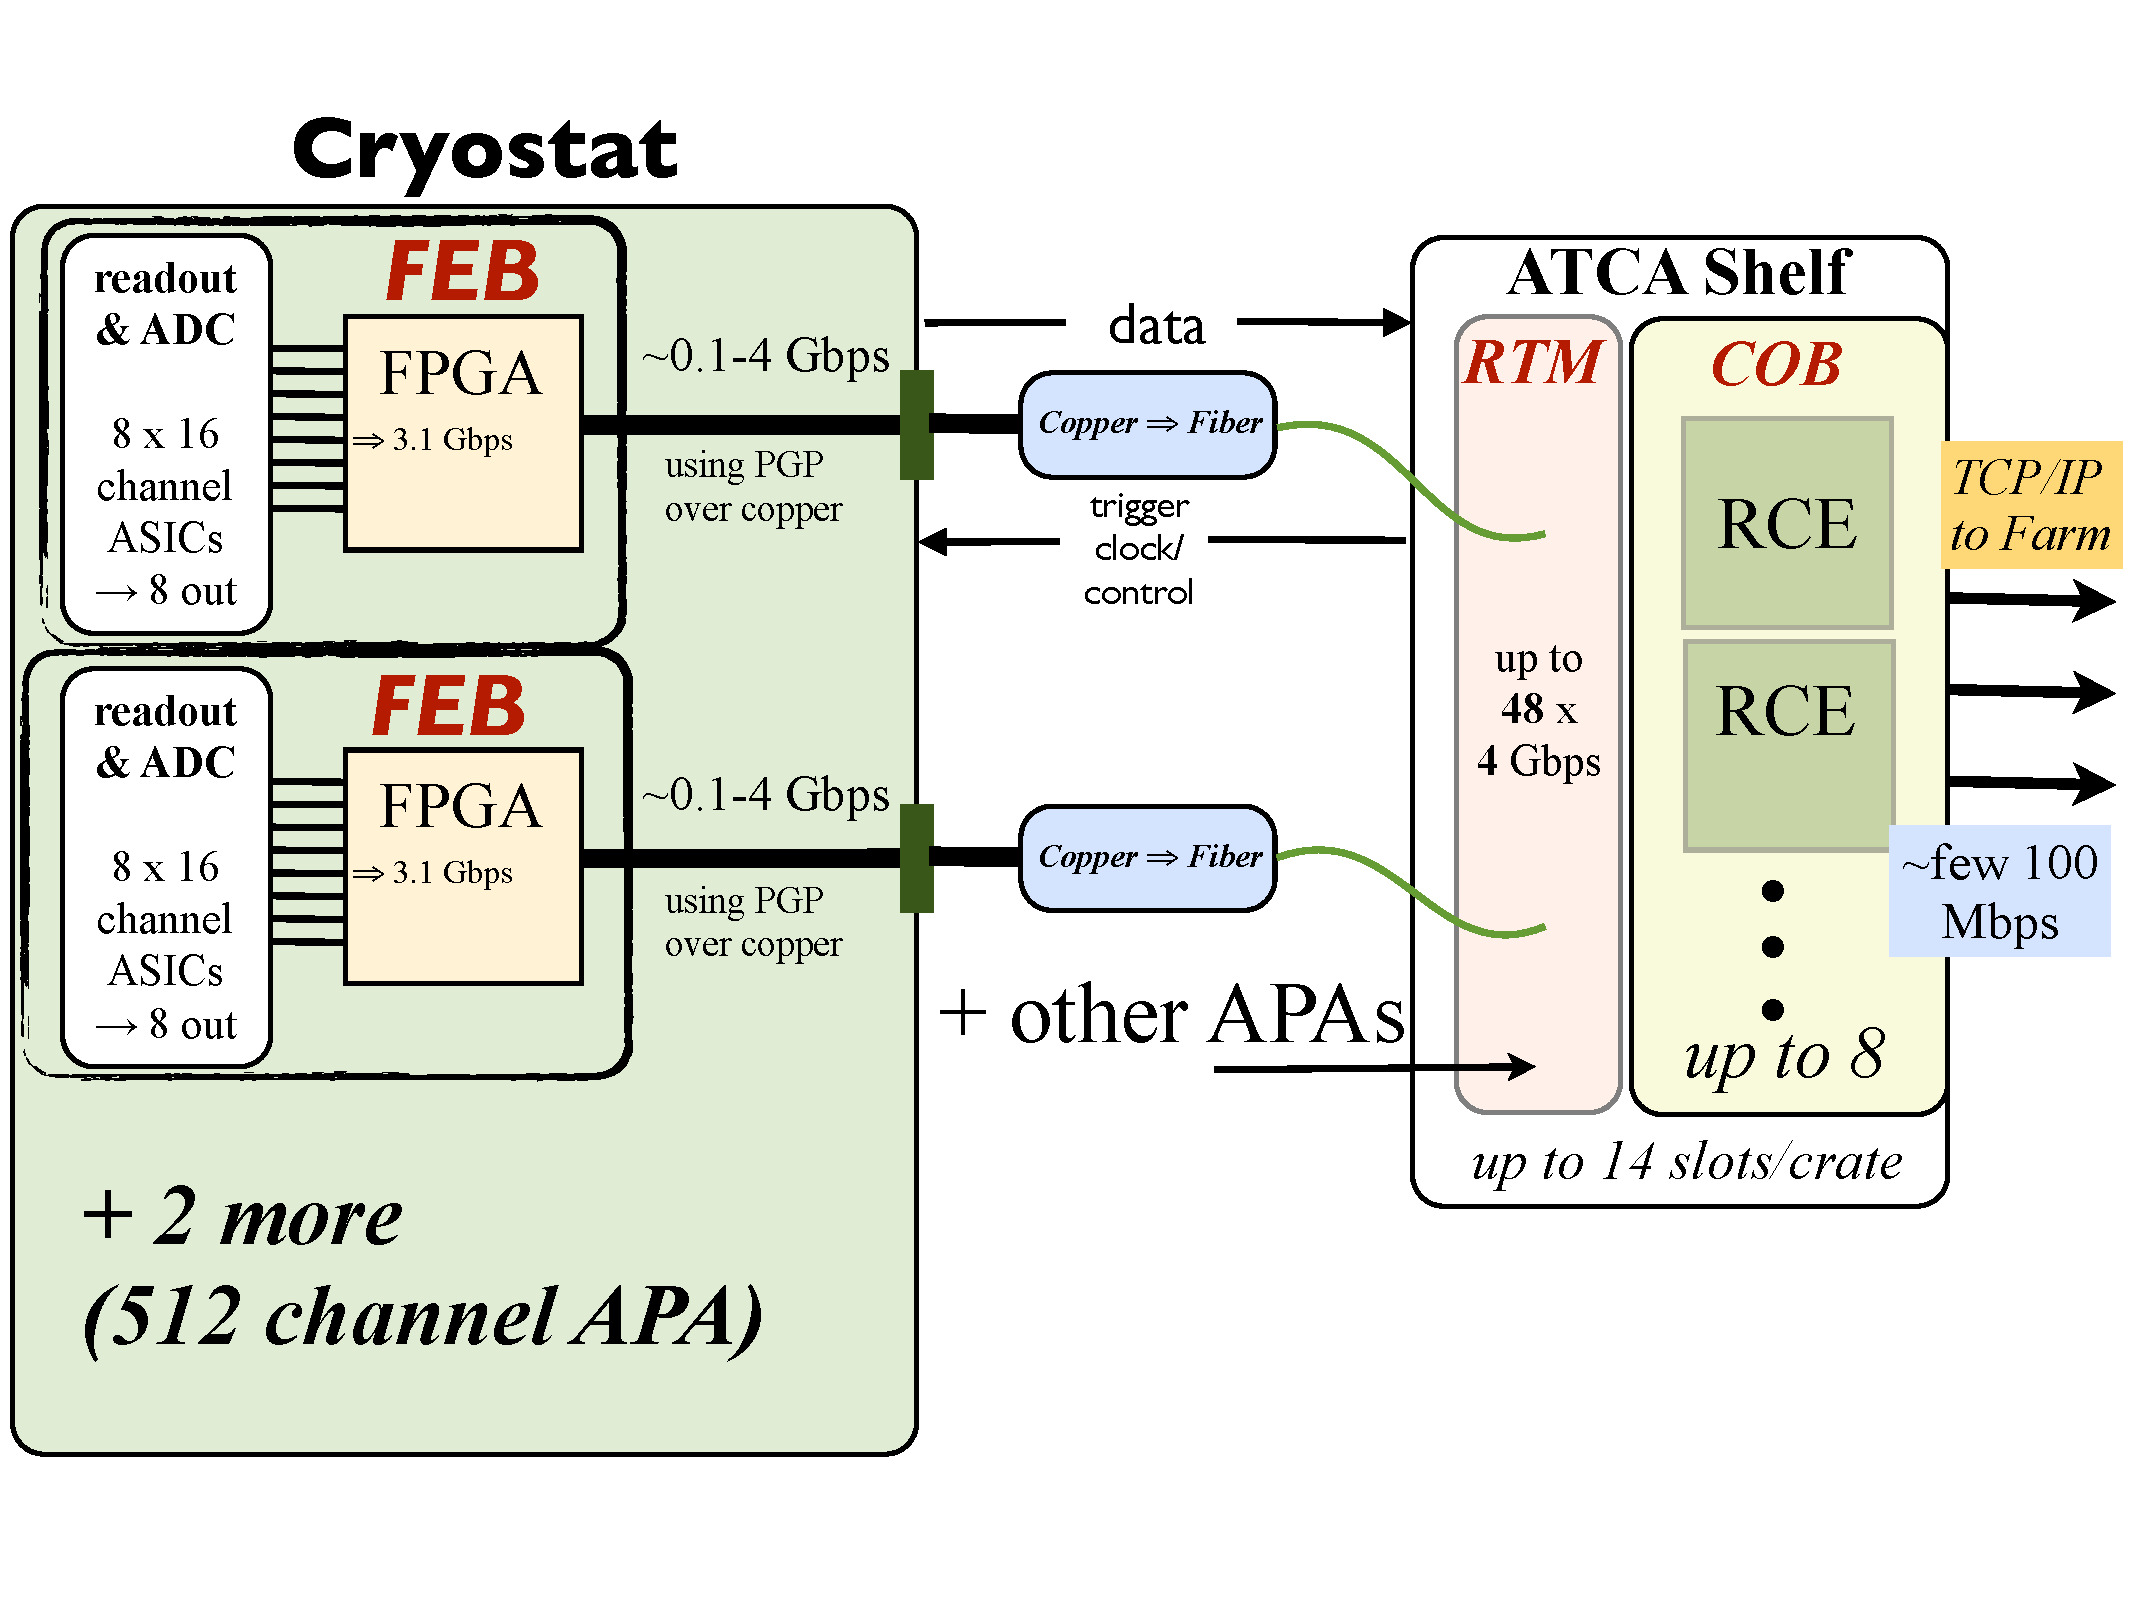
\includegraphics[scale=0.6,angle=90]{LBNE-DAQ-BlockDiagram.pdf}
\caption{Block diagram of the RCE-based DAQ for a single TPC APA.}
\label{fig:blockDiag}
\end{figure} 


%================
\begin{table}[tbh]
\begin{center}
\begin{tabular}{|l|c|c|}   
\hline \hline 
    & 35t  & Full LBNE \\      
\hline
   Total Channels        & $\sim$2k &$\sim$307k \\ 
	Number of APAs     &  4 (?)     &    120        \\ 
   Number of FEBs       & 16 & 2400 \\ 
   Transition Boards    & 16(???) & 2400(????) \\ 
   RTM+COB Boards    & 1   &  50 \\
   ATCA Crates            & 1   &  4 (14-slot)   \\ 
\hline \hline
\end{tabular}
\caption[]{DAQ-related quantities for the 35t and full LBNE (as of Jan. 2013 design).}
\label{tab:daqsumm} 
\end{center}
\end{table}
%=================


\subsection{Full LBNE}

....  assumptions, schematic of DAQ chain, summary of what/how many of each component we need  ....  


..."transition boards" are the copper->fiber boards...maybe these are in the flange itself...for full LBNE, would make sense to do some multiplexing here (maybe 20:4 ... go from an APA, single cable/FEB to a 4-fiber cable???)


\subsection{Phase 2 of 35t Prototype}


....  assumptions, schematic of DAQ chain, summary of what/how many of each component we need  ....  


\subsection{Comparision of RCE-based vs DCM-based Backend DAQ Systems}

... list of the many ways RCE-based system is so much better  ....

\subsection{High-speed Data Links From Cold FPGA to Backend DAQ}

...possibilities and our plans on this ...


\subsection{DAQ Test-stand}


